\documentclass[12pt, a4paper]{book}
\usepackage{authblk, fancyhdr, hyperref, multirow, graphicx, subfig, longtable}
\hypersetup{
    colorlinks,
    citecolor=black,
    filecolor=black,
    linkcolor=black,
    urlcolor=black
}
\usepackage[left=25mm,right=25mm,top=25mm,bottom=25mm]{geometry}
\usepackage{listings}
\usepackage{amssymb}

\newcommand\Chapter[2]{
  \chapter[#1: {\itshape#2}]{#1\\[2ex]\Large\itshape#2}
}
\usepackage{lipsum}
\pagestyle{headings}

\title{Parallel Computation Summary}
\author{Moatasem Gamal}
\affil{FCAI BSU}

\begin{document}
\maketitle
\tableofcontents
\chapter{Multithreaded Programming}
\section{Introduction}
\begin{itemize}
    \item Modern operating systems hold more than one activity (program) in memory and the processor can switch among all to execute them.
    \item \textbf{Multitasking/MultiProcesses:} is the simultaneous occurrence of several activities (program) on a computer.
    \item Actually to have true multitasking, the applications run on a machine with multiple processors.
    \item Multitasking results in effective and simultaneous utilization of various system resources such as processors, disks, and printers.
\end{itemize}
\section{Parallel Programming vs Sequential Programming}
\begin{itemize}
    \item In parallel programming, multiple tasks are executed simultaneously, allowing for better performance and maximum utilization of system resources such as processors, disks, and printers.
    \item Sequential Programming means that process are executed sequentially, one after another. When running a sequential Java program, commands are executed linearly, where each process must complete before the next one starts.
\end{itemize}

\section{The operating system multitasking}
The operating system supports multitasking in a \textbf{cooperative} or \textbf{preemptive} manner.
\subsection{Cooperative manner}
In cooperative multitasking each application is responsible for relinquishing control to the processor to enable it to execute the other application, as in earlier versions of operating systems.
\subsection{Preemptive manner}
In the preemptive type multitasking, the processor is responsible for executing each application in a certain amount of time called a time slice, as in modern operating systems.
\subsection{Cooperative VS Preemptive}
table (\ref{tab:cooperativeVsPreemptive}) shows the main differences between the two manners\\
\begin{table}[!ht]
    \centering
    \begin{tabular}{|c|p{0.6\linewidth}|p{0.20\linewidth}|}
        \hline
        Manner                       & responsibility                                                                                                                   & used in                               \\
        \hline
        \multirow{2}{*}{Cooperative} & \textbf{application} $\rightarrow$ relinquishing control to the \textbf{processor} to enable it to execute the other application & earlier versions of operating systems \\
        \hline
        \multirow{2}{*}{Preemptive}  & \textbf{processor} $\rightarrow$ executing each application in a certain amount of time called a  \textbf{time slice}            & modern operating systems              \\
        \hline
    \end{tabular}
    \label{tab:cooperativeVsPreemptive}
    \caption{Cooperative VS Preemptive}
\end{table}
\\
Note: A single processor computer is shared among multiple applications with preemptive multitasking, the processor is switching between the applications at intervals of milliseconds, you feel that all applications run concurrently.
\section{Concepts: Process and Thread}
% \begin{table}[h]
\begin{longtable}{c|p{0.45\linewidth}|p{0.45\linewidth}}
                                    & \Large{Process}                                                                                        & \Large{Thread}                                                                                                                                                    \\
    \hline
    \rotatebox{-90}{Definition}     & \begin{itemize}
                                          \item A process is a program in execution
                                          \item A process is sometime referred as task
                                          \item A process is a collection of one or more threads and associated system resources.
                                          \item A process may be divided into a number of independent units known as threads
                                          \item A process may have a number of threads in it.
                                      \end{itemize}                & \begin{itemize}
                                                                         \item Threads are light-weight processes within a process
                                                                         \item A thread is a dispatchable unit of work
                                                                         \item A thread may be assumed as a subset of a process.
                                                                         \item A thread is a smallest part of the process that can execute concurrently with other parts(threads) of the process
                                                                     \end{itemize}                                                                                                                      \\
    \hline
    \rotatebox{-90}{Multitasking }  &
    \begin{itemize}
        \item Multitasking of two or more processes is known as  \textbf{process-based multitasking}
        \item Process-based multitasking is totally controlled by the \textbf{operating system}
    \end{itemize}
                                    &
    \begin{itemize}
        \item Multitasking of two or more threads is known as \textbf{thread-based multitasking}
        \item The concept of multithreading in a programming language refers to thread-based multitasking
        \item thread-based multitasking can be controlled by the \textbf{programmer} to some extent in a program
    \end{itemize}
    \\
    \hline
    \rotatebox{-90}{Address Space } & A process has its own address space                                                                    & A thread uses the process’s address space and share it with the other threads of that process                                                                     \\
    \hline
    \rotatebox{-90}{Communication } & A process can communicate with other process by using inter-process communication                      & \begin{itemize}
                                                                                                                                                   \item A thread can communicate with other thread (of the same process) directly by using methods like wait(), notify(), notifyAll().
                                                                                                                                                   \item All threads within a process share the same state and same memory space, and can communicate with each other directly, because they share the same variables
                                                                                                                                               \end{itemize} \\
    \hline
    \rotatebox{-90}{New Creation }  & the creation of new processes require duplication of the parent process                                & New threads are easily created                                                                                                                                    \\
    \hline
    \rotatebox{-90}{Control }       & A process does not have control over the sibling process, it has control over its child processes only & Threads have control over the other threads of the same process                                                                                                   \\
    \hline
    \rotatebox{-90}{Construct }     & Processes are an architectural construct                                                               & Thread is a coding construct that does not affect the architecture of an application
\end{longtable}
% \caption{Process VS Thread}
% \end{table}
\subsection{Process containing single and multiple threads}
\begin{figure}[!h]
    \centering
    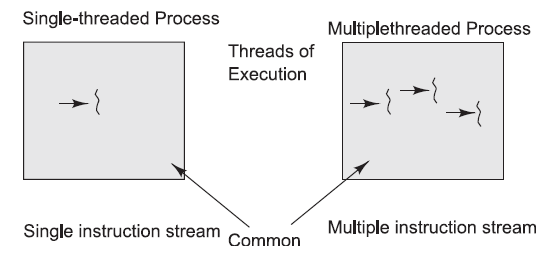
\includegraphics[width=0.7\linewidth]{figures/process-containing-threads.png}
\end{figure}
\subsection{The advantages of thread-based multitasking as compared to process-based multitasking :}
\begin{itemize}
    \item Threads share the same address space.
    \item  Context-switching between threads is normally inexpensive.
    \item Communication between threads is normally inexpensive.
    \item Java supports thread-based multitasking.
\end{itemize}
\section{Context Switching}
\begin{itemize}
    \item The concept of context switching is integral to threading.
    \item A hardware timer is used by the processor to determine the end of the time-slice for each thread.
    \item The timer signals at the end of the timeslice and in turn the processor saves all information required for the current thread onto a \textbf{stack}. Then the processor moves this information from the stack into a predefined data structure called a \textbf{context structure}.
    \item When the processor wants to switch back to a previously executing thread, it transfers all the information from the context structure associated with the thread to the stack.
\end{itemize}

\chapter{THREADS IN JAVA}
We focus on learning how to write an application containing multiple tasks that can be executed concurrently. In Java, this is realized by using multithreading techniques.\\
\section{Threads}
\begin{itemize}
    \item All threads within a process share the same state and same memory space, and can communicate with each other directly, because they share the same variables.
    \item A single process might contain multiple threads.
    \item Java supports thread-based multitasking
    \item Threads are lightweight processes as the overhead of switching between threads is less
    \item They can be easily spawned
    \item The Java Virtual Machine (JVM) spawns a thread when your program is run called the Main Thread
    \item Multiple Threads on single CPU or multiple CPUs:\begin{figure}[!h]
              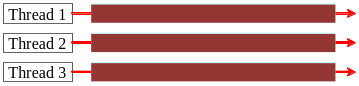
\includegraphics[width=0.4\linewidth]{figures/Multiple-threads-on-multiple-CPUs.png}
              Multiple Threads on multiple CPUs
              \\ ----------------------------------------------------------------------- \\
              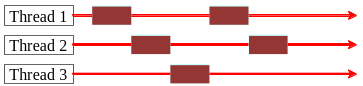
\includegraphics[width=0.4\linewidth]{figures/Multiple-threads-sharing-a-single-CPU.png}
              Multiple threads sharing a single CPU
          \end{figure}
    \item Program with master and children threads \begin{figure}[!h]
              \centering
              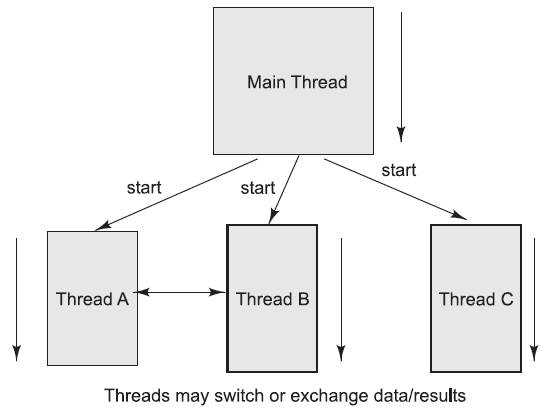
\includegraphics[width=0.6\linewidth]{figures/Program-with-master-and-children-threads.png}
          \end{figure}
\end{itemize}
\subsection{Why do we need threads?}
\begin{itemize}
    \item To  enhance parallel processing
    \item To increase response to the user
    \item To utilize the idle time of the CPU
    \item Prioritize your work depending on priority
\end{itemize}
\section{Implementing Threads in Java}
\begin{itemize}
    \item Threads are objects in the Java language. They can be created by using two different mechanisms:
          \begin{enumerate}
              \item Create a class that \textbf{extends} the standard \textbf{Thread} class.
              \item Create a class that \textbf{implements} the standard \textbf{Runnable} interface
          \end{enumerate}
          \begin{figure}[!h]
              \centering
              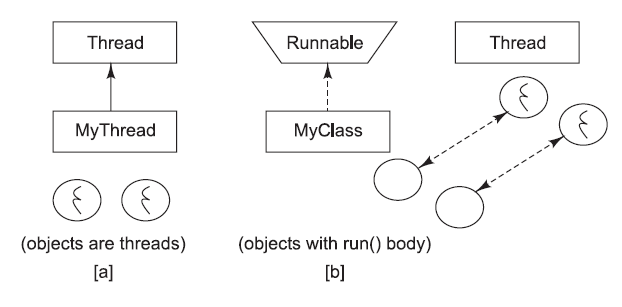
\includegraphics[width=0.8\linewidth]{figures/threads-in-java.png}
          \end{figure}

    \item Thread can be defined by:
          \begin{itemize}
              \item Extending the java.lang.Thread class, or
              \item Implementing the java.lang.Runnable interface.
          \end{itemize}
    \item The run() method should be overridden and should contain the code that will be executed by the new thread.
          This method must be public with a void return type and should not take any arguments.
    \item run() method is the starting point for thread execution
\end{itemize}
\subsection{Extending the Thread Class}
\begin{enumerate}
    \item  Create a class by extending the Thread class and override the run() method:
          \begin{lstlisting}[language=java]
class MyThread extends Thread {
    public void run() {
	    // thread body of execution
    }
}
    \end{lstlisting}
    \item Create a thread object:
          \begin{lstlisting}[language=java]
MyThread thr1 = new MyThread();
    \end{lstlisting}
    \item Start Execution of created thread: \begin{lstlisting}[language=java]
thr1.start();
    \end{lstlisting}
\end{enumerate}
\textbf{Example} \\
\begin{lstlisting}[language=java]
/* ThreadEx1.java: A simple program creating and invoking a thread object 
by extending the standard Thread class. */
class MyThread extends Thread {
    public void run() {
        System.out.println(" this thread is running ... ");
    }
}
class ThreadEx1 {
    public static void main(String [] args ) {
        MyThread t = new MyThread();
        t.start();
    }
}
\end{lstlisting}
\subsection{Implementing the Runnable Interface}
It is more preferred to implement the Runnable Interface so that we can extend properties from other classes
\begin{enumerate}
    \item Create a class that implements the interface Runnable and override run() method:
          \begin{lstlisting}[language=java]
class MyThread implements Runnable {
    ...
    public void run() {
        // thread body of execution
    }
}
    \end{lstlisting}
    \item Creating Object:
          \begin{lstlisting}[language=java]
        MyThread myObject = new MyThread();
    \end{lstlisting}
    \item Creating Thread Object:
          \begin{lstlisting}[language=java]
        Thread thr1 = new Thread(myObject);
    \end{lstlisting}
    \item Start Execution:
          \begin{lstlisting}[language=java]
        thr1.start();
    \end{lstlisting}
\end{enumerate}
\textbf{Example} \\
\begin{lstlisting}[language=java]
/* ThreadEx2.java: A simple program creating and invoking a thread object by
implementing Runnable interface. */
class MyThread implements Runnable {
    public void run() {
        System.out.println(" this thread is running ... ");
    }
}
class ThreadEx2 {
    public static void main(String [] args ) {
        Thread t = new Thread(new MyThread());
        t.start();
    }
}
\end{lstlisting}
\section{Life cycle of threads \& Thread states}
\subsection{Life Cycle of Thread}
\begin{figure}[!h]
    \centering
    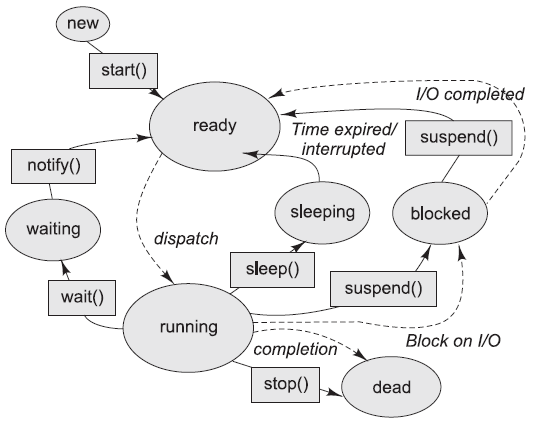
\includegraphics[width=0.9\linewidth]{figures/Life-cycle-of-Java-threads.png}
\end{figure}
\subsection{Thread States}
\begin{figure}[!h]
    \centering
    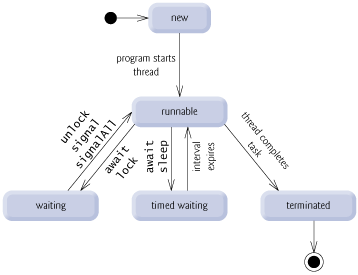
\includegraphics[width=0.9\linewidth]{figures/thread-states.png}
\end{figure}

A thread can be in one of five states: New, Ready, Running, Blocked, or Finished showed in figure(\ref{fig:thread-states-detaild}).
\begin{figure}[!h]
    \centering
    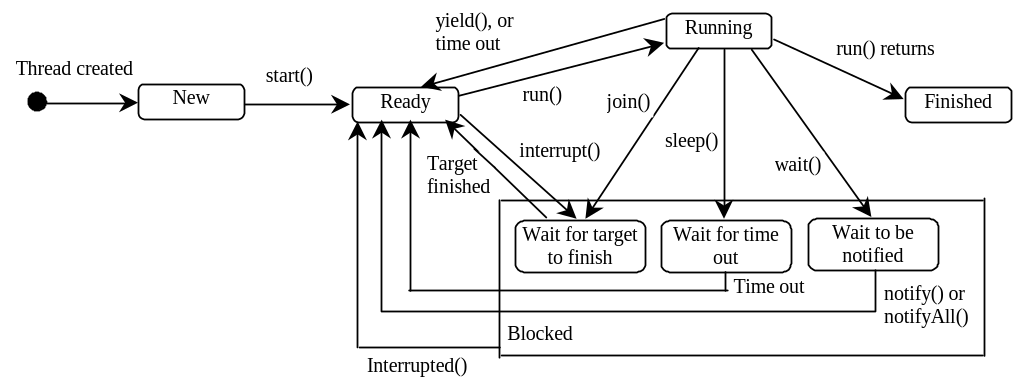
\includegraphics[width=0.9\linewidth]{figures/thread-states-detaild.png}
    \label{fig:thread-states-detaild}
    \caption{Thread states}
\end{figure}

\subsection{Thread termination}
A thread becomes Not Runnable when one of these events occurs:
\begin{itemize}
    \item  Its sleep method is invoked.
    \item  The thread calls the wait method to wait for a specific condition to be satisfied.
    \item  The thread is blocking on I/O.
\end{itemize}
\section{Good example}
\begin{itemize}
    \item Consider a simple web server
    \item    The web server listens for request and serves it
    \item If the web server was not multithreaded, the requests processing would be in a queue, thus increasing the response time and also might hang the server if there was a bad request.
    \item By implementing in a multithreaded environment, the web server can serve multiple request simultaneously thus improving response time
\end{itemize}
\section{Running threads}
\begin{lstlisting}[language=java]
class mythread implements Runnable{
    public void run(){
        System.out.println("Thread Started");
    }
}

class mainclass {
    public static void main(String args[]){
        Thread  t = new Thread(new mythread()); // This is the way to instantiate a 					 thread implementing runnable interface
        t.start(); // starts the thread by running the run method
    }
}
\end{lstlisting}
\begin{itemize}
    \item Calling t.run() does not start a thread, it is just a simple method call.
    \item Creating an object does not create a thread, calling start() method creates the thread.
\end{itemize}

\section{Synchronization}
\begin{itemize}
    \item Synchronization is prevent data corruption
    \item Synchronization allows only one thread to perform an operation on a object at a time.
    \item If multiple threads require an access to an object, synchronization helps in maintaining consistency.
\end{itemize}
\subsection{Example on Synchronization}
\begin{lstlisting}[language=java]
public class Counter{
    private int count = 0;
    public int getCount(){
        return count;
    }

    public setCount(int count){
        this.count = count;
    }
}
\end{lstlisting}
\begin{itemize}
    \item In this example, the counter tells how many an access has been made.
    \item If a thread is accessing setCount and updating count and another thread is accessing getCount at the same time, there will be inconsistency in the value of count.
\end{itemize}
\subsubsection{Fixing the example}
\begin{lstlisting}[language=java]
public class Counter{
	private static int count = 0;
	public synchronized int getCount(){
		return count;
	}

	public synchoronized setCount(int count){
    	this.count = count;
	}
}
\end{lstlisting}
\begin{itemize}
    \item By adding the synchronized keyword we make sure that when one thread is in the setCount method the other threads are all in waiting state.
\end{itemize}
\subsection{What about static methods?}
\begin{lstlisting}[language=java]
public class Counter{
	private int count = 0;
	public static synchronized int getCount(){
	    return count;
	}

	public static synchronized setCount(int count){
	    this.count = count;
	}
}
\end{lstlisting}
\begin{itemize}
    \item In this example the methods are static and hence are associated with the class and not the instance.
    \item Hence the lock is placed on the class object that is, Counter.class object and not on the object itself.  Any other non static synchronized methods are still available for access by other threads.
\end{itemize}
\subsection{Common Synchronization mistake}
\begin{lstlisting}[language=java]
public class Counter{
	private int count = 0;
	public static synchronized int getCount(){
		 return count;
	}

	public synchronized setCount(int count){
		this.count = count;
	}
}
\end{lstlisting}
\begin{itemize}
    \item The common mistake here is one method is static synchronized and another method is non static synchronized.
    \item This makes a difference as locks are placed on two different objects. The class object and the instance and hence two different threads can access the methods simultaneously.
\end{itemize}
\subsection{Synchronization vs Static Synchronization}

\begin{tabular}{c|p{0.35\linewidth}|p{0.35\linewidth}}
    Feature                    & \textbf{Synchronization}                                                                & \textbf{Static Synchronization}                                                                     \\
    \hline
    Scope                      & Object-level                                                                            & Class-level                                                                                         \\
    \hline
    Lock Acquisition           & Acquires lock on the object instance                                                    & Acquires lock on the class itself                                                                   \\
    \hline
    Impact on Multiple Objects & Each object's synchronized methods can be accessed by different threads simultaneously. & Only one thread can access any static synchronized method of the class at a time.                   \\
    \hline
    Usage                      & Used to protect shared resources at the object level                                    & Used to protect shared resources at the class level or for operations that involve the class itself \\
    \hline
    Declaration                & Applied to instance methods using the synchronized keyword                              & Applied to static methods using the static synchronized keywords                                    \\
    \hline
    Example                    & public synchronized void deposit() { ... }                                              & public static synchronized void getInstance() { ... }                                               \\
\end{tabular}
\chapter{Parallel Computing: Overview (PSC)}{by John Urbanicurbanic@psc.edu}
\section{Why we need parallel computing?}
for \textbf{New Applications} \\
The graph shows that applications that require processing large amounts of data are the ones that benefit most from parallel computing.
\begin{figure}[!h]
    \centering
    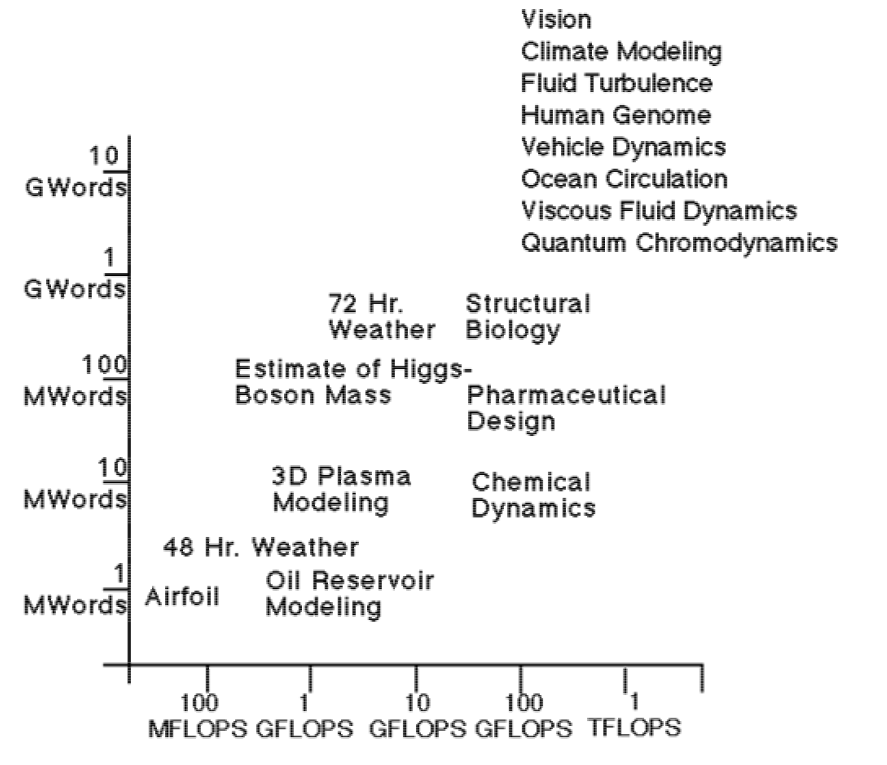
\includegraphics[width=0.7\linewidth]{figures/new-applications.png}
\end{figure}
\begin{itemize}
    \item The performance capabilities of supercomputers are expressed using a standard rate for indicating the number of floating-point arithmetic calculations systems can perform on a per-second basis. The rate, \textbf{floating-point operations per second}, is abbreviated as \textbf{FLOPS}.
    \item The per-second rate "FLOPS" is commonly misinterpreted as the plural form of "FLOP" (short for "floating-point operation") \cite{flops}
\end{itemize}
\section{Clock Speed}
\subsection{clock speed over previous years}
\begin{figure}[!h]
    \centering
    \subfloat{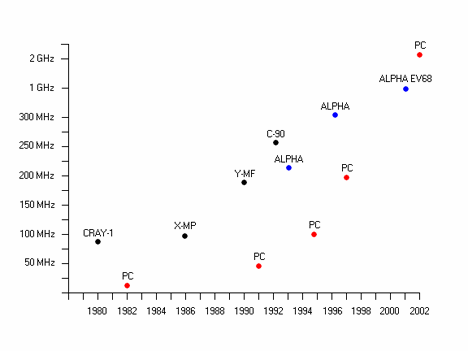
\includegraphics[width=0.55\linewidth]{figures/clock-speeds01.png}}
    \subfloat{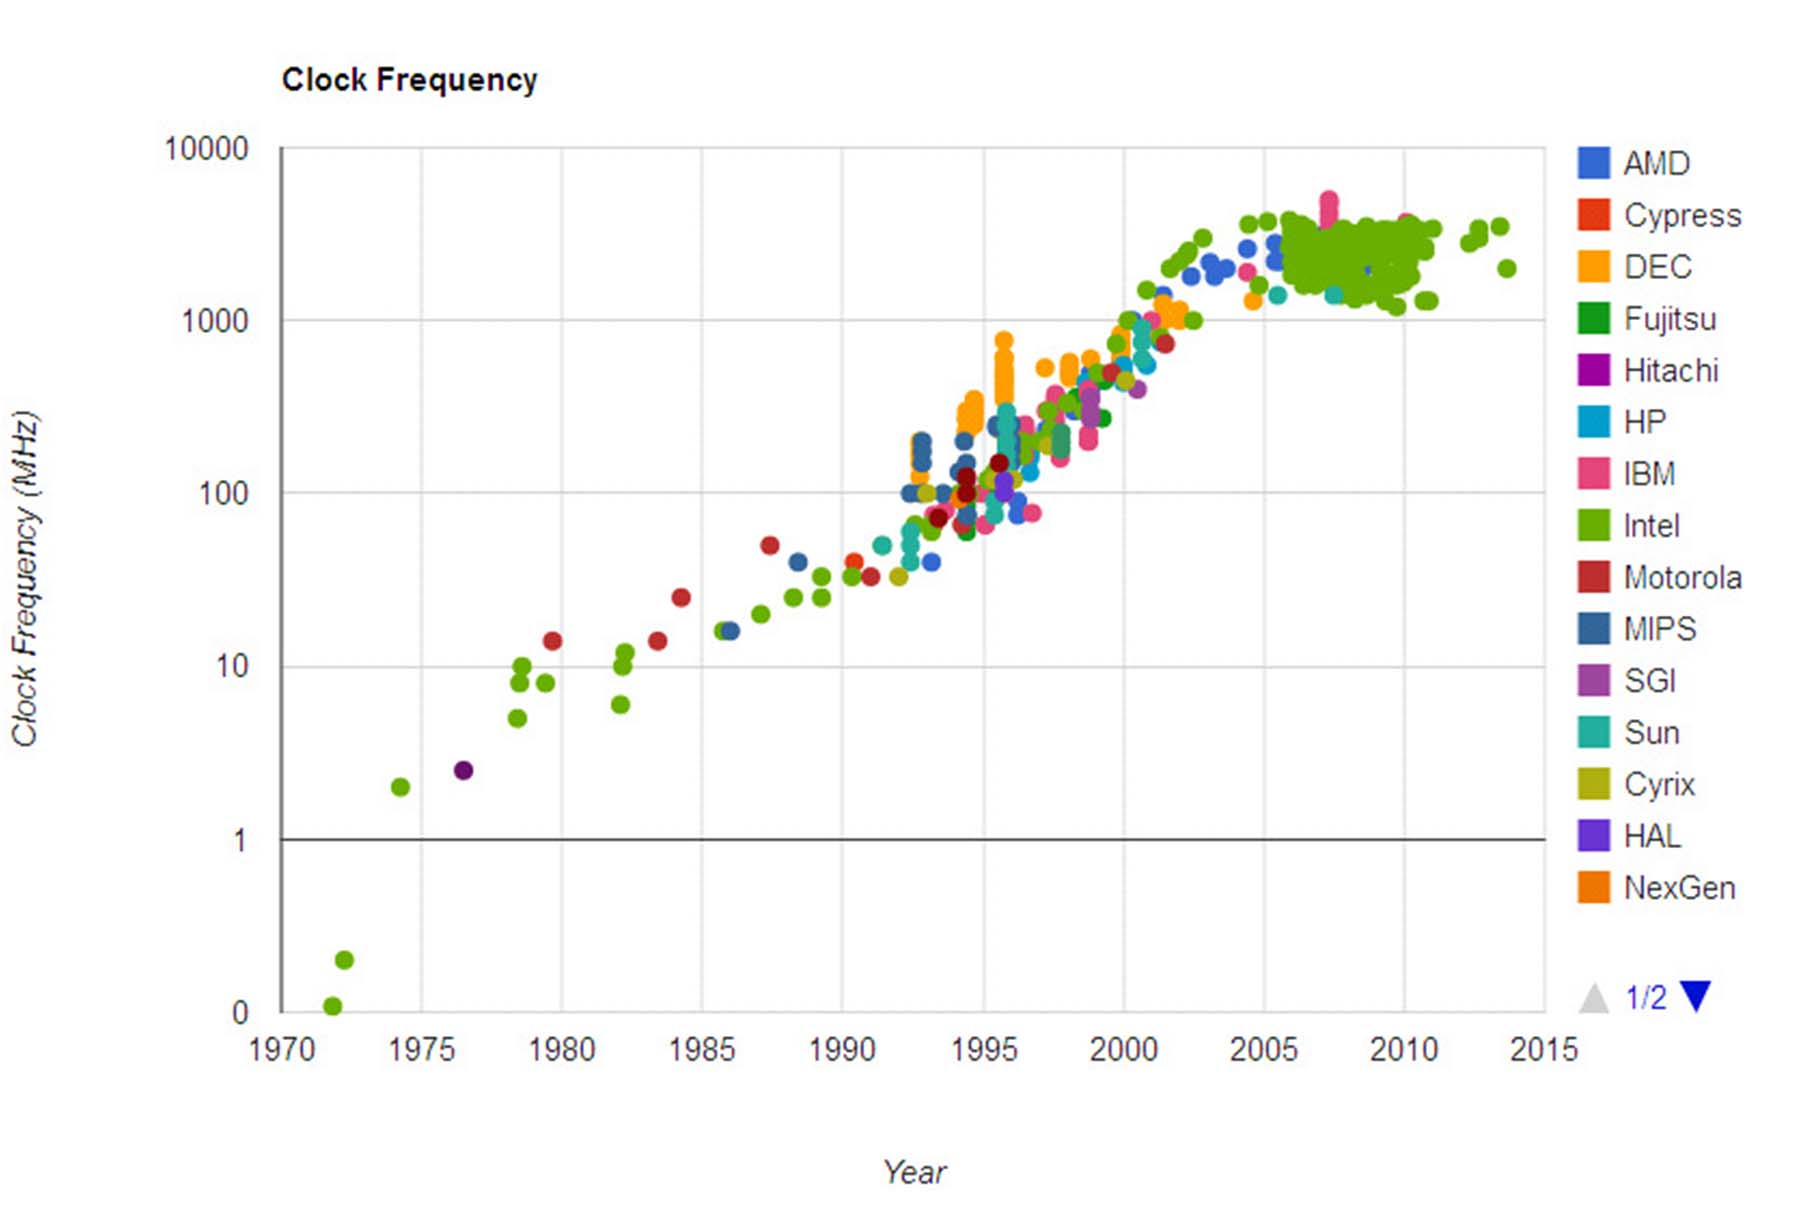
\includegraphics[width=0.55\linewidth]{figures/clock-speeds02.png}}
\end{figure}

\subsection{Y-MP vs C90 supercomputers}
When the PSC \footnote{PSC ~ Pittsburgh Supercomputing Center, The Pittsburgh Supercomputing Center (PSC) is a high performance computing and networking center founded in 1986 and one of the original five NSF Supercomputing Centers.} went from a 2.7 GFlop Y-MP
to a 16 GFlop C90, the clock only got 50%
faster. The rest of the speed increase was
due to increased use of parallel techniques:
\begin{itemize}
    \item More processors (8 $\rightarrow$ 16)
    \item Longer vector pipes (64 $\rightarrow$ 128)
    \item Parallel functional units (2)
\end{itemize}

\begin{table}[h]
    \centering
    \begin{tabular}{l|c|c}
        --                        & Y-MP & C90 \\
        \hline
        processors                & 8    & 16  \\
        \hline
        vector pipes              & 64   & 128 \\
        \hline
        Parallel functional units & 2    & 2   \\
    \end{tabular}
\end{table}

So, we want as many processors working
together as possible. How do we do this?
There are two distinct elements:
\begin{itemize}
    \item Hardware: vendor does this
    \item Software: you, at least today
\end{itemize}

\section{Amdahl's Law}
How many processors can we really use? \\

\begin{minipage}{0.6\linewidth}
    Let's say we have a legacy
    code such that is it only
    feasible to convert half of
    the heavily used routines
    to parallel:
    \begin{itemize}
        \item If we run this on a parallel
              machine with five processors:
              Our code now takes about
              60s. We have sped it up
              by about 40\%.
        \item Let's say
              we use a thousand
              processors:
              We have now sped our code
              by about a factor of two.
    \end{itemize}
\end{minipage}
\hfill
\begin{minipage}{0.3\linewidth}
    \centering
    \begin{tabular}{|c|c|}
        \hline
        25s & Serial   \\
        \hline
        50s & Parallel \\
        \hline
        25s & Serial   \\
        \hline
    \end{tabular}
    \\
    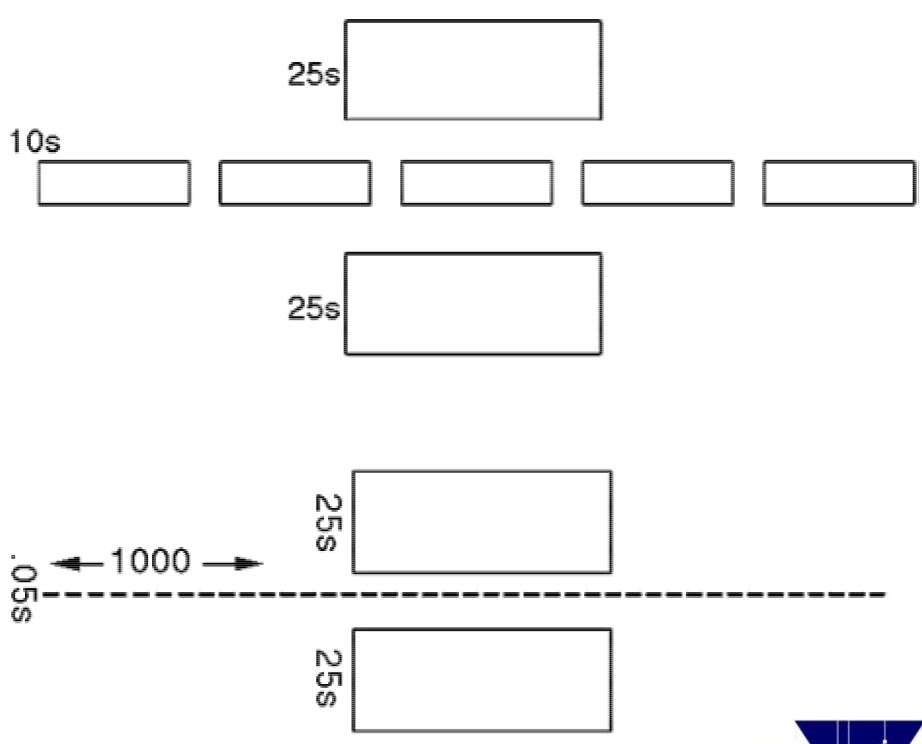
\includegraphics[width=0.99\linewidth]{figures/amdahl-law02.png}
\end{minipage}
% \begin{minipage}{0.6\linewidth}

% \end{minipage}
% \hfill
% \begin{minipage}{0.4\linewidth}
% \end{minipage}

This seems pretty depressing, and it does point out one limitation of converting old
codes one subroutine at a time. However, most new codes, and almost all parallel
algorithms, can be written almost entirely in parallel (usually, the “start up” or
initial input I/O code is the exception), resulting in significant practical speed ups.
This can be quantified by how well a code scales which is often measured as
efficiency.
\begin{figure}[!h]
    \centering
    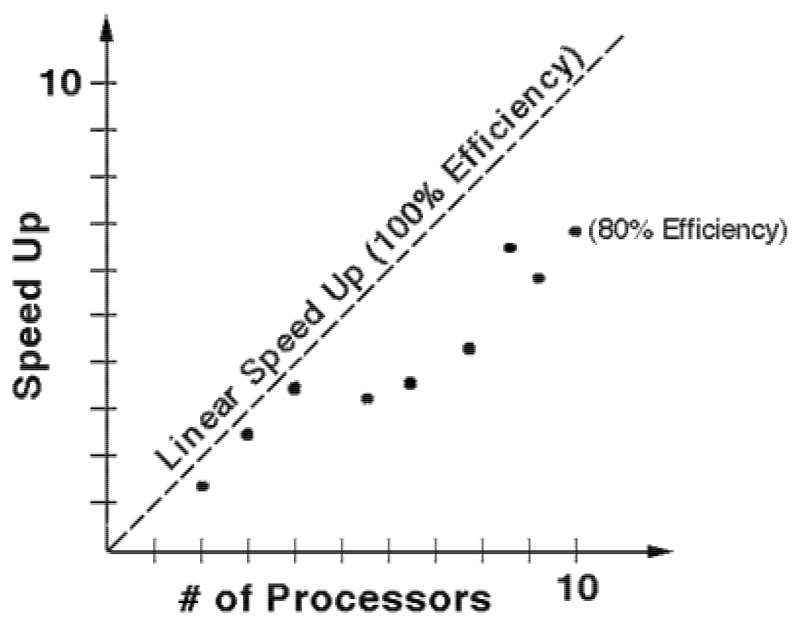
\includegraphics[width=0.5\linewidth]{figures/amdahl-law03.png}
\end{figure}
\subsection{Amdahl's Law equation}
\subsubsection{Time}
if single-processor finishes one program in one unit of time, how much time will multiple-processors require to finish that task?\\
\begin{equation}
    Time_{for\ 1\ processor} = 1
\end{equation}
\begin{equation}
    Time_{for\ 2\ processor} = \frac{1}{2}
\end{equation}
\begin{equation}
    Time_{for\ n\ processors} = \frac{1}{n}
\end{equation}
\subsubsection{Speedup}
If you are using n processors, your $Speedup_n$ is:
\begin{equation}
    Speedup_n = \frac{T_1}{T_n}
\end{equation}
And your Speedup $\mathrm{Efficiency_n}$ is:
\begin{equation}
    \mathrm{Efficiency_n} = \frac{Speedup_n}{n}
\end{equation}
which could be as high as 1., but probably never will be.
\subsubsection{Amdahl's law}
If you put in n processors, you should get n times Speedup
(and 100\% Speedup Efficiency), right? Wrong!
There are always some fraction of the total operation that is inherently
sequential and cannot be parallelized no matter what you do. This includes
reading data, setting up calculations, control logic, storing results, etc. \\ \\
If you think of all the operations that a program needs to do as being
divided between a fraction that is parallelizable and a fraction that isn't
(i.e., is stuck at being sequential), then Amdahl's Law says:

\begin{equation}
    Speedup_n = \frac{T_1}{T_n} = \frac{1}{\frac{F_{parallel}}{n}+F_{sequential}} = \frac{1}{\frac{F_{parallel}}{n}+(1-F_{parallel})}
\end{equation}

\subsubsection{Maximum Possible SpeedUp}
\begin{equation}
    max\ Speedup = \frac{1}{1-F_{parallel}}
\end{equation}
\subsubsection{Example 1}
5\% of a parallel programs's execution time is spent within inherently sequential code.
Calculate The maximum speedup achievable by this program, regardless of how many PEs are used \\
Solution \\
\begin{equation}
    Speedup_\infty = \frac{1}{\frac{0.95}{\infty}+0.05} = 20
\end{equation}
\subsubsection{Example 2}
95\% of a program's execution time occurs inside a loop
that can be executed in parallel. What is the maximum
speedup we should expect from a parallel version of the
program executing on 8 CPUs? \\
Solution \\
\begin{equation}
    Speedup_8 = \frac{1}{\frac{0.95}{8}+0.05} \approx 5.9
\end{equation}
\section{Shared Memory and Distributed Memory}
\subsection{Shared Memory}
\begin{minipage}{0.65\linewidth}
    Easiest to program. There are no
    real data distribution or
    communication issues. Why
    doesn't everyone use this
    scheme?
    \begin{itemize}
        \item Limited numbers of processors
              (tens) - Only so many
              processors can share the same
              bus before conflicts dominate.
        \item Limited memory size -
              Memory shares bus as well.
              Accessing one part of memory
              will interfere with access to
              other parts.
    \end{itemize}
\end{minipage}
\hfill
\begin{minipage}{0.3\linewidth}
    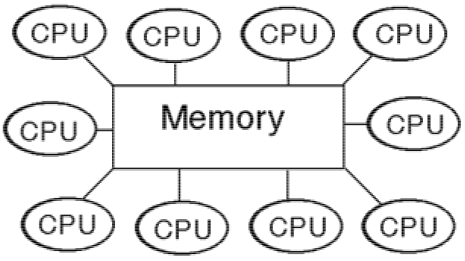
\includegraphics[width=0.99\linewidth]{figures/shared-memory01.png}
    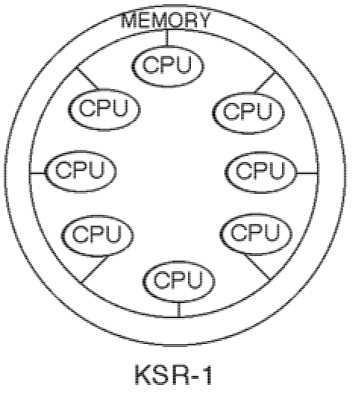
\includegraphics[width=0.99\linewidth]{figures/shared-memory02.png}
\end{minipage}
\begin{table}[h!]
    \centering
    \caption{Comparison of Shared and Distributed Memory Architectures}
    \label{tab:shared_distributed}
    \begin{tabular}{|l|c|c|}
        \hline
        \textbf{Feature}     & \textbf{Shared Memory} & \textbf{Distributed Memory}                   \\ \hline
        Ease of Programming  & Easier                 & More difficult                                \\ \hline
        Data Distribution    & Not required           & Crucial                                       \\ \hline
        Communication Issues & Minimal                & Significant                                   \\ \hline
        Number of Processors & Limited (tens)         & Limited by physical size (tens of meters)     \\ \hline
        Memory Size          & Limited                & Very large                                    \\ \hline
        Local Disk per Node  & Often available        & Usually not available                         \\ \hline
        Virtual Memory       & Supported              & Not typically supported                       \\ \hline
        Data Access Times    & Uniform                & Dependent on data location (local vs. remote) \\ \hline
    \end{tabular}
\end{table}

\section{}
\subsection{Common Distributed Memory Machines}
\section{Latency and Bandwidth}
\section{Data Parallel}
\section{Work Sharing}
\section{Load Balancing}
\bibliography{./ref}
\bibliographystyle{plain}
\end{document}